\subsection{Qualitative observations on connectome properties}
We first inspected the connectome matrix of a clinically normal individual for an overview of typical connectivity patterns (\autoref{fig:connectome_cn_0_full}). Interhemispheric edges appear sparser than intrahemispheric connections, in line with known neuroanatomical pathways mostly confined to one hemisphere except for crossing through the corpus callosum. The cerebellum cortex exhibits relatively strong cross‐hemisphere connections, likely attributable to the bilateral layout of cerebellar peduncles. 

\begin{figure}[H]
    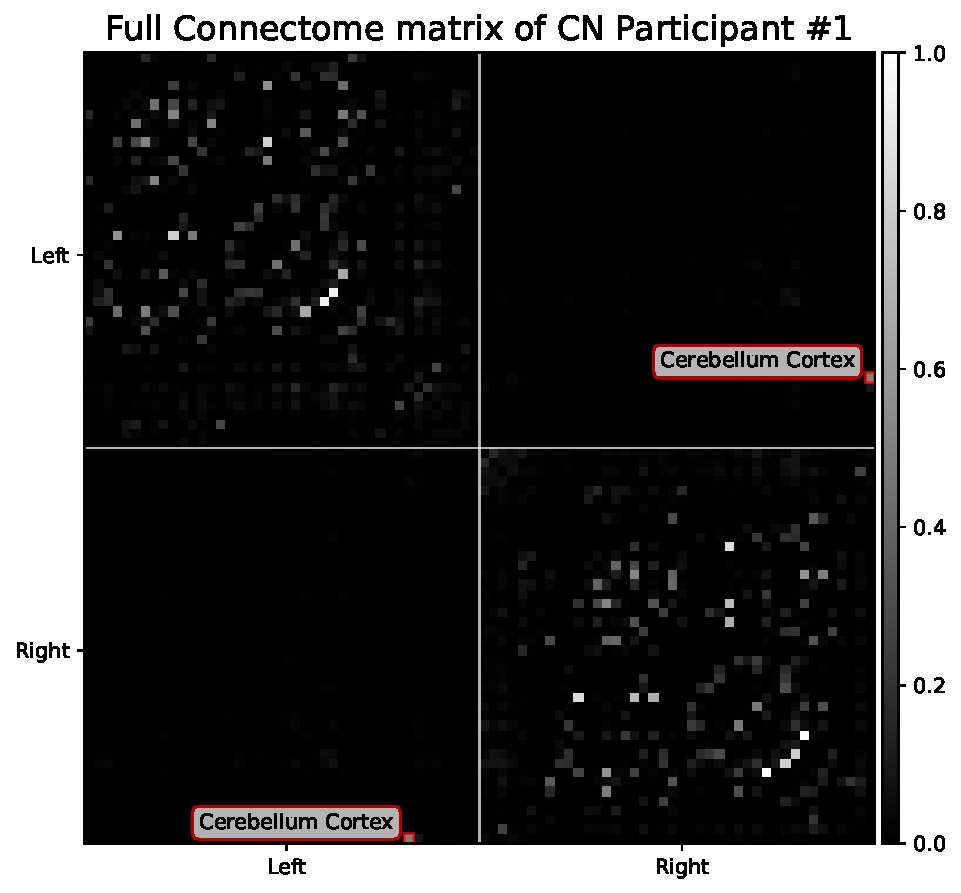
\includegraphics[width=0.8\linewidth]{figures/connectome_cn_0_full.pdf}
    \caption{Full connectome matrix.}
    \label{fig:connectome_cn_0_full}
\end{figure}

\begin{figure}[H]
    \centering
    \begin{subfigure}[a]{\linewidth}
      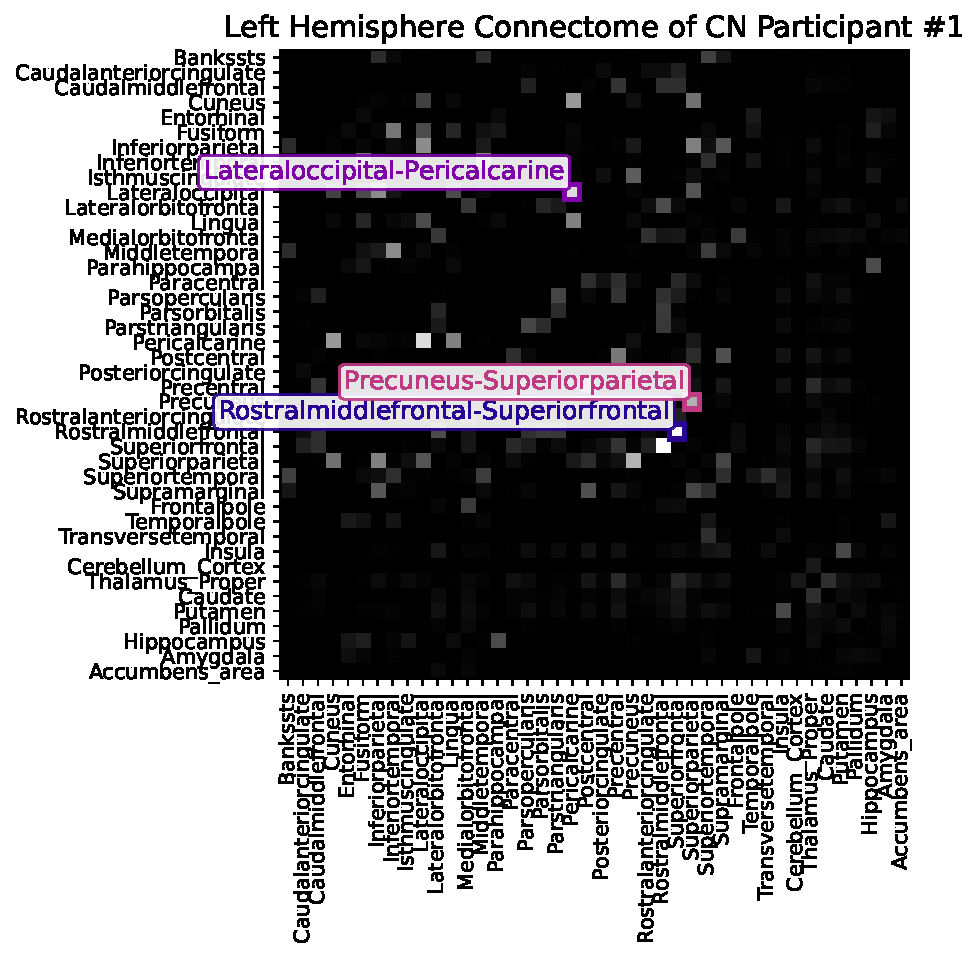
\includegraphics[width=\linewidth]{figures/connectome_cn_0_left.pdf}
      \caption{Left hemisphere.}
      \label{fig:connectome_cn_0_left}
    \end{subfigure}
    \vskip 1ex
    \begin{subfigure}[b]{\linewidth}
      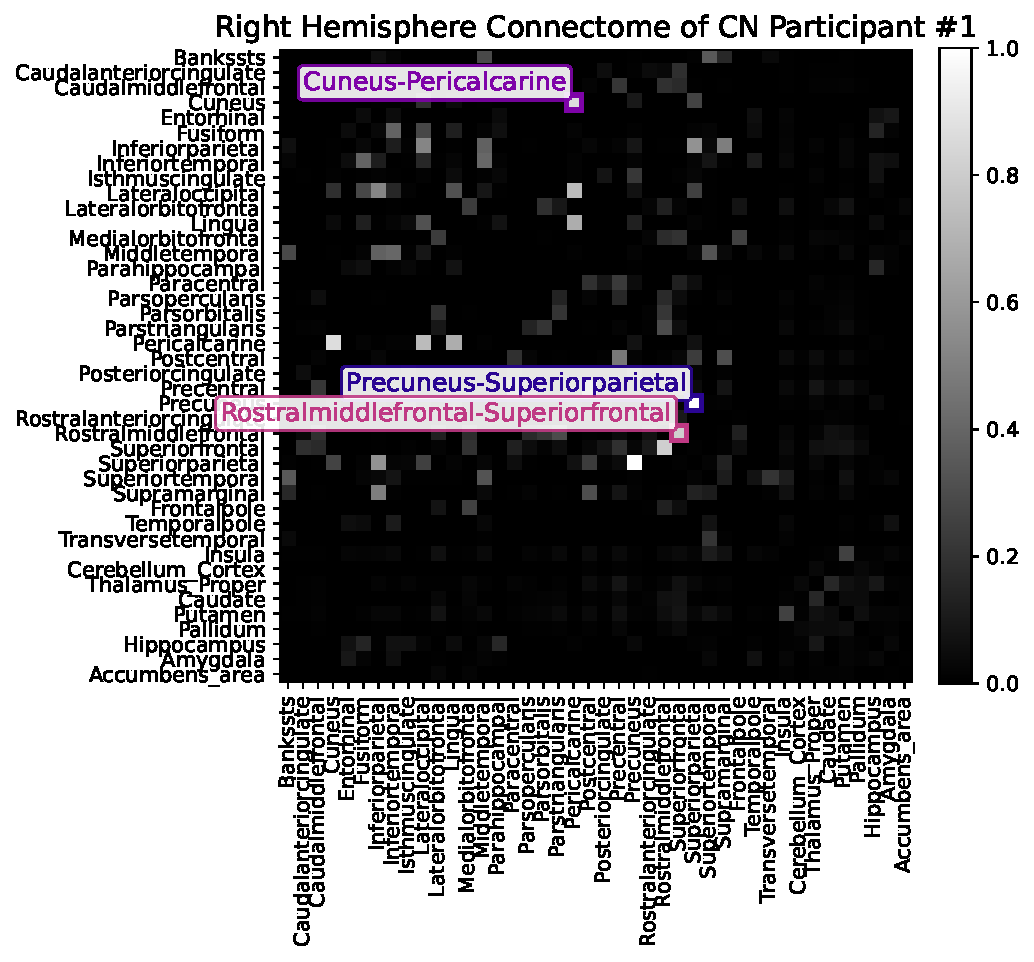
\includegraphics[width=\linewidth]{figures/connectome_cn_0_right.pdf}
      \caption{Right hemisphere.}
      \label{fig:connectome_cn_0_right}
    \end{subfigure}
    \caption{Combined connectome visualisations for a clinically normal participant.}
    \label{fig:connectome_cn_0}
\end{figure}

We then observed intra-hemispheric connectivity. Within the left hemisphere (\autoref{fig:connectome_cn_0_left}), the strongest edges link Cuneus-Pericalcarine, Precuneus-Superiorparietal and Postcentral-Precentral. We observe similar patterns in the right hemisphere (\autoref{fig:connectome_cn_0_right}), with strongest edges connecting Rostralmiddlefrontal-Superiorfrontal, Cuneus-Pericalcarine and Precuneus-Superiorparietal.

    
\begin{figure*}[b]
    \centering
    % The figure part
    \begin{tcolorbox}[colback=white, colframe=black, boxrule=0.5pt, arc=0pt]
        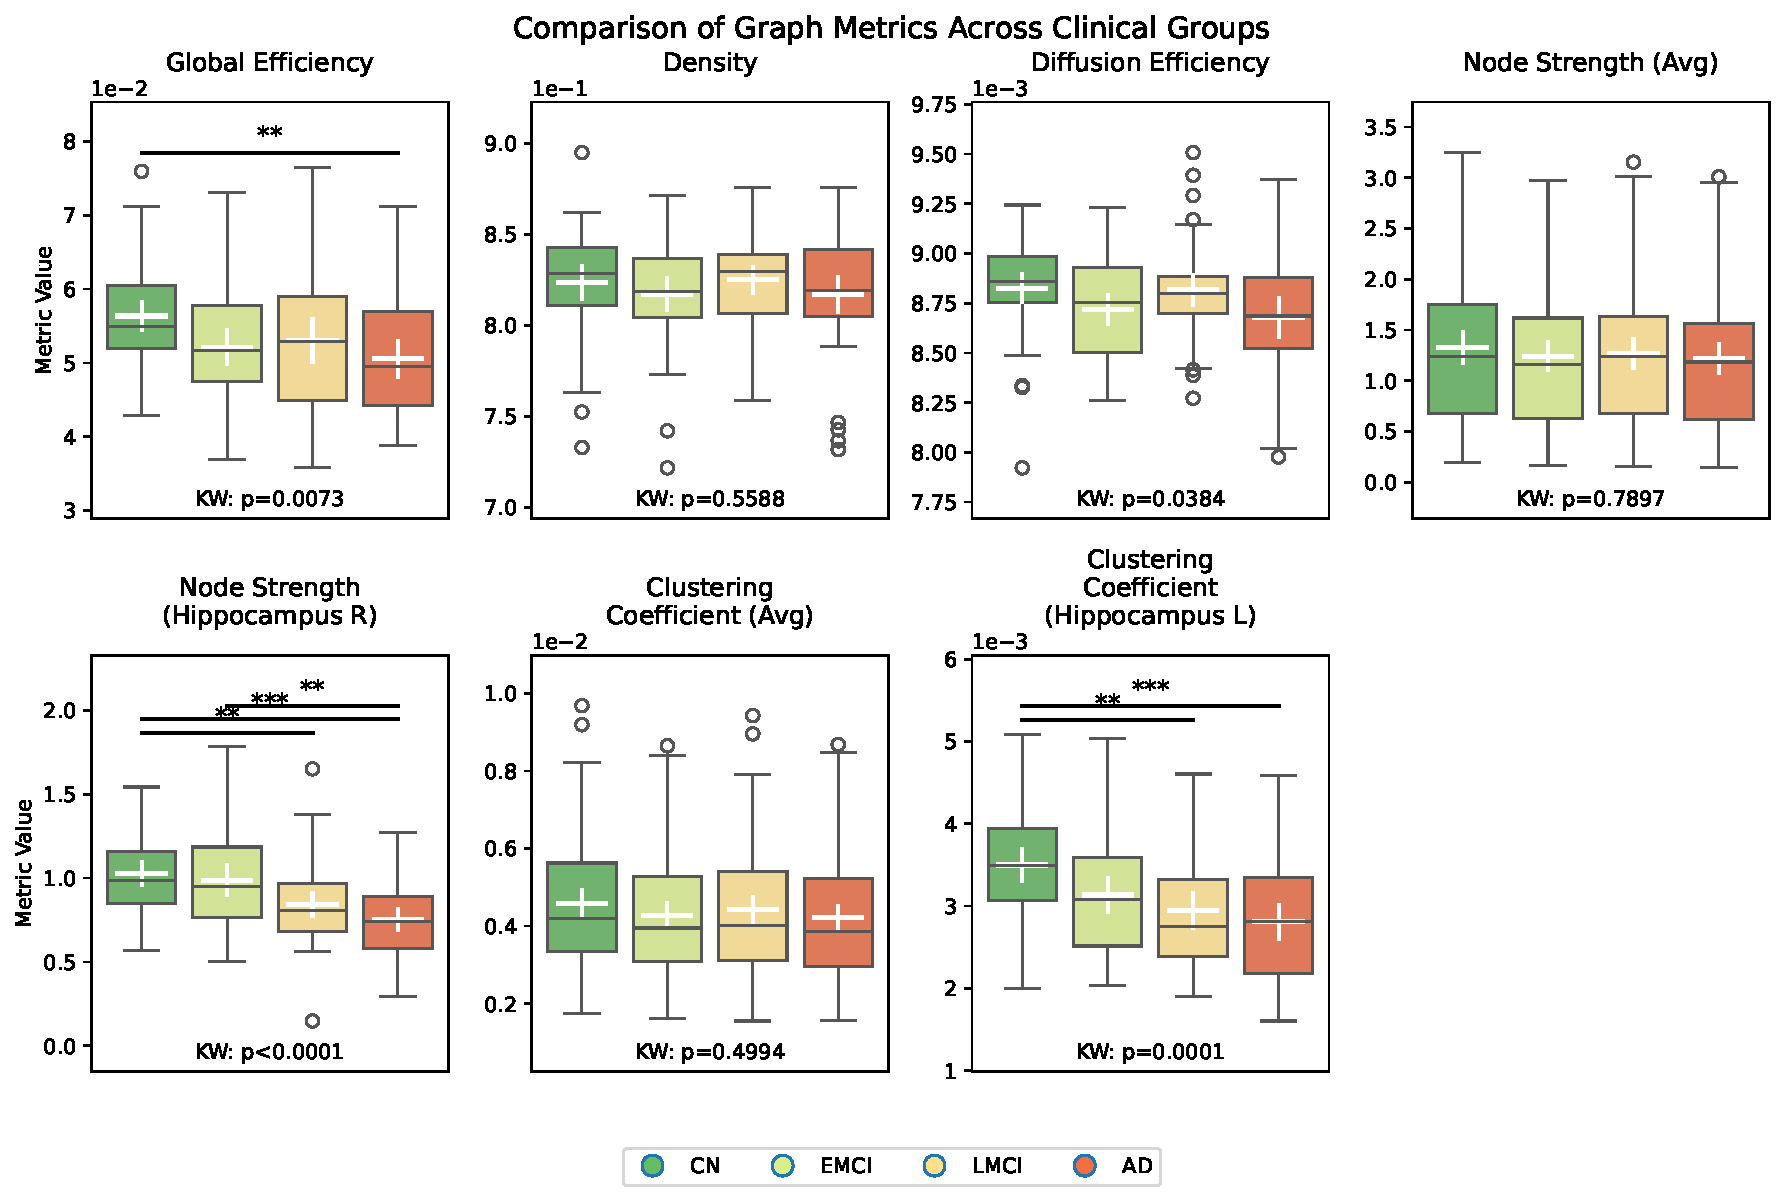
\includegraphics[width=\textwidth]{figures/graph_metrics_comparison.pdf}
        \caption{Connectome metrics for different cognitive stages. White horizontal lines indicate the group mean and vertical lines indicate the 95\% confidence intervals. Kruskal-Wallis p-values are annotated at the bottom and pairwise differences are computed using Dunn's post-hoc test. Significance indicators: * denotes p $<$ 0.05, ** denotes p $<$ 0.01, and *** denotes p $<$ 0.001.}
    
    
    \label{fig:graph_metrics_comparison}
    
    \vskip 4mm
    % The table part (without table environment)
    \small
    \captionof{table}{Significant pairwise comparisons between clinical groups}
    \label{tab:significant_comparisons}
    \begin{tabular}{lllrrrc}
        \toprule
        \textbf{Metric} & \textbf{Group 1} & \textbf{Group 2} & \textbf{Mean 1} & \textbf{Mean 2} & \textbf{\% Diff} & \textbf{p-value} \\
        \midrule
        Global Efficiency & CN & DEM & 5.64e-02 & 5.05e-02 & -10.3\% & 0.004 \\
        Node Strength (Hippocampus R) & CN & LMCI & 1.03e+00 & 8.43e-01 & -17.9\% & 0.005 \\
        Node Strength (Hippocampus R) & CN & DEM & 1.03e+00 & 7.52e-01 & -26.8\% & $<$0.001 \\
        Node Strength (Hippocampus R) & EMCI & DEM & 9.88e-01 & 7.52e-01 & -23.9\% & 0.001 \\
        Clustering Coefficient (Hippocampus L) & CN & LMCI & 3.50e-03 & 2.94e-03 & -15.9\% & 0.002 \\
        Clustering Coefficient (Hippocampus L) & CN & DEM & 3.50e-03 & 2.81e-03 & -19.7\% & $<$0.001 \\
        \bottomrule
    \end{tabular}
\end{tcolorbox}
\end{figure*}

\subsection{Connectome properties vary across different cognitive stages}\label{section:connectome_metrics_results}
We compared the connectome metrics as mentioned in \autoref{section:connectome_metrics}. 
We comment below on the metrics that show significant differences in the Dunn posthoc tests.
\begin{itemize}
    \item \textbf{Global Efficiency}: Shows significant decline (p=0.0073) as cognitive impairment progresses, with particularly strong differences between CN and AD groups (**). This suggests diminishing network integration capacity with disease progression. 
    \item \textbf{Node Strength (Right-Hippocampus)}: Displays the strongest statistical significance (p$<$0.0001) with clear stepwise decline from CN to AD, marked by multiple significant pairwise comparisons (**). This aligns with known hippocampal vulnerability in Alzheimer's disease.
    \item \textbf{Clustering Coefficient (Left-Hippocampus)}: Shows significant differences (p=0.0001) with a pronounced decrease in the AD group, indicating reduced local connectivity in this key memory-related region.
\end{itemize}




% \begin{figure*}[b]
%     \centering
%     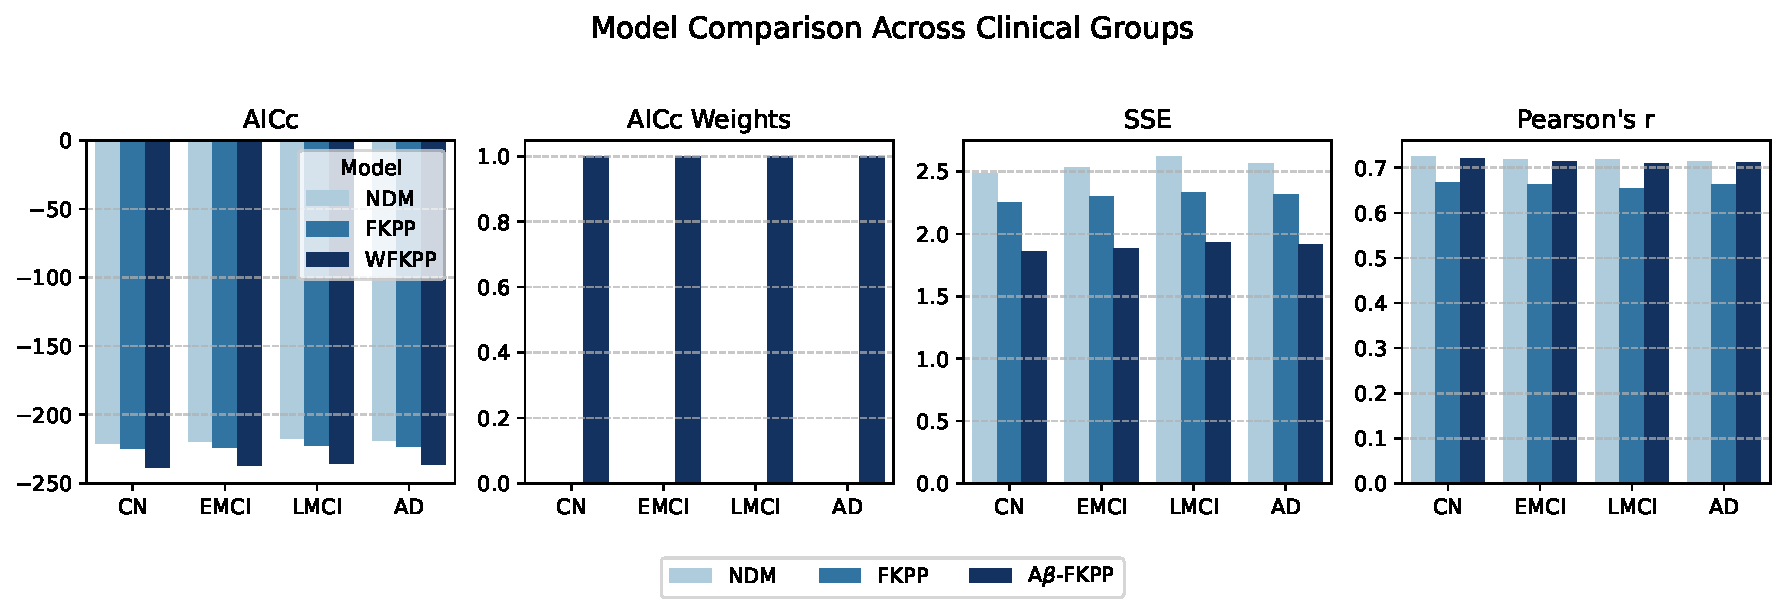
\includegraphics[width=1\linewidth]{figures/model_comparison.pdf}
%     \caption{Comparison of model performance across different cognitive stages.}
%     \label{fig:model_comparison}
% \end{figure*}

% In your preamble, ensure you have:
% \usepackage{caption}  % or \usepackage{capt-of}

\begin{figure*}[tbp]
    \begin{tcolorbox}
        \centering
        % --- Top row: main comparison figure ---
        \begin{subfigure}{\linewidth}
            \centering
            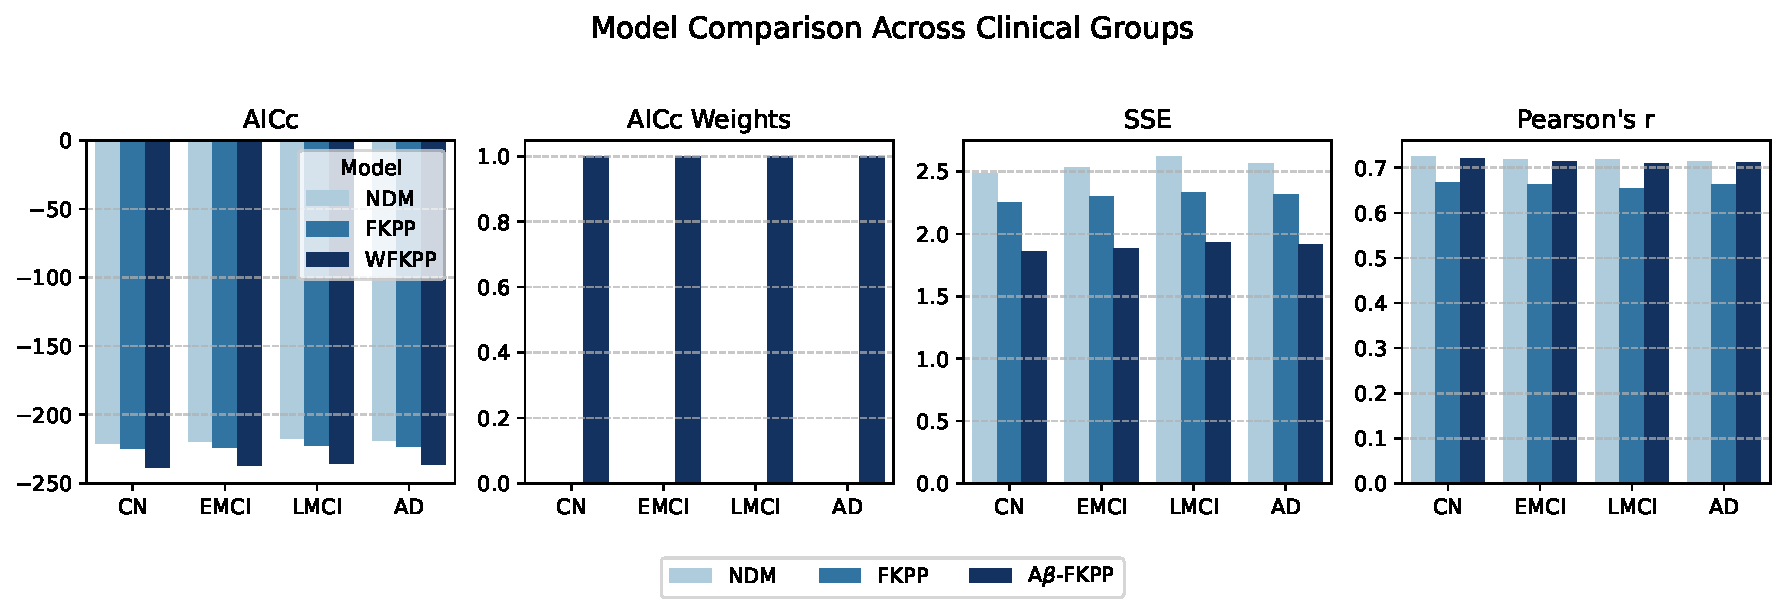
\includegraphics[width=\linewidth]{figures/model_comparison.pdf}
            \caption{Comparison of model performance across different models and cognitive stages.}
            \label{fig:model_comparison_main}
        \end{subfigure}
        
        \vspace{2em} % space before second row
        
        % --- Second row: residual plots ---
        \begin{subfigure}{0.32\linewidth}
            \centering
            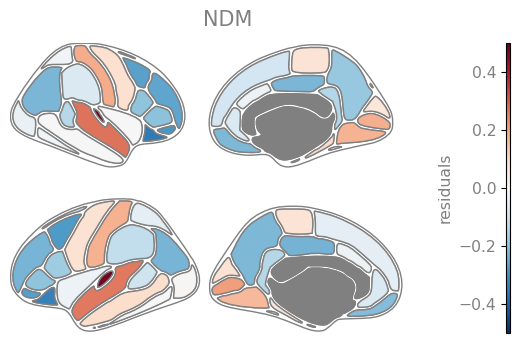
\includegraphics[width=\linewidth]{residuals_ndm_cn.png}
            \caption{NDM residuals}
            \label{fig:ndm_residuals}
        \end{subfigure}
        \hfill
        \begin{subfigure}{0.32\linewidth}
            \centering
            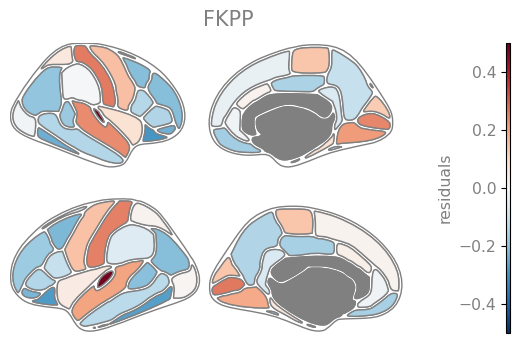
\includegraphics[width=\linewidth]{residuals_fkpp_cn.png}
            \caption{FKPP residuals}
            \label{fig:fkpp_residuals}
        \end{subfigure}
        \hfill
        \begin{subfigure}{0.32\linewidth}
            \centering
            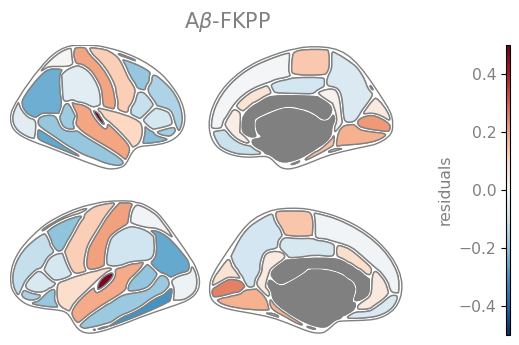
\includegraphics[width=\linewidth]{residuals_wfkpp_cn.png}
            \caption{A$\beta$-FKPP residuals}
            \label{fig:wfkpp_residuals}
        \end{subfigure}
        
        \vspace{1.5em} % Space before third row
        
        % --- Third row: correlation plots ---
        \begin{subfigure}{\linewidth}
            \centering
            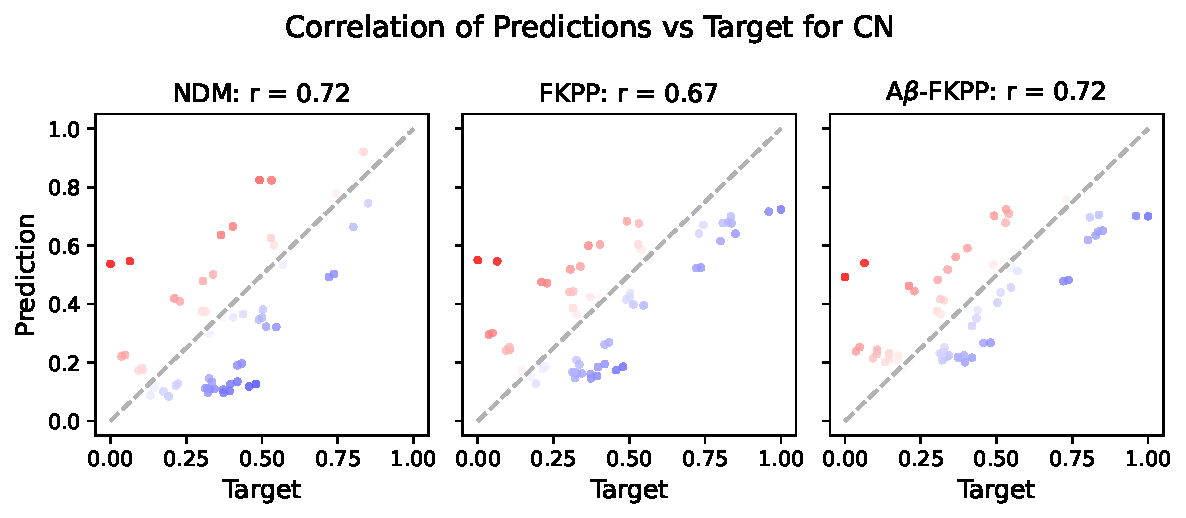
\includegraphics[width=\linewidth]{figures/correlation_prediction_vs_target_cn.pdf}
            \caption{Prediction vs target for NDM, FKPP, and A$\beta$-FKPP models in CN.}
            \label{fig:correlation_plots}
        \end{subfigure}
        
        \vspace{1.5em} % Space before fourth row
        
        % --- Fourth row: table ---
        \begin{subfigure}{\linewidth}
            \centering
            \begin{tabular}{c|p{4.5cm}|p{4.5cm}|p{4.5cm}}
                \toprule
                 & \textbf{NDM} & \textbf{FKPP} & \textbf{WFKPP} \\
                \midrule
                \multirow{3}{*}{\rotatebox[origin=c]{90}{\textbf{Over}}} &
                \textcolor{red}{Transversetemporal R} &
                \textcolor{red}{Transversetemporal R} &
                \textcolor{red}{Transversetemporal R} \\
                & \textcolor{red}{Transversetemporal L} &
                \textcolor{red}{Transversetemporal L} &
                \textcolor{red}{Transversetemporal L} \\
                & \textcolor{red}{Temporalpole R} &
                \textcolor{red}{Pericalcarine L} &
                \textcolor{red}{Pericalcarine L} \\
                \midrule
                \multirow{3}{*}{\rotatebox[origin=c]{90}{\textbf{Under}}} &
                \textcolor{blue}{Lateralorbitofrontal R} &
                \textcolor{blue}{Lateralorbitofrontal R} &
                \textcolor{blue}{Inferiortemporal L} \\
                & \textcolor{blue}{Lateralorbitofrontal L} &
                \textcolor{blue}{Lateralorbitofrontal L} &
                \textcolor{blue}{Inferiortemporal R} \\
                & \textcolor{blue}{Parsorbitalis R} &
                \textcolor{blue}{Inferiortemporal L} &
                \textcolor{blue}{Inferiorparietal L} \\
                \bottomrule
            \end{tabular}
            \caption{Regions with largest prediction errors across models in CN group}
            \label{fig:error_regions_table}
        \end{subfigure}
    \end{tcolorbox}
    \caption{Comprehensive comparison of model performance, residuals, and prediction errors.}
    \label{fig:model_comparison}
\end{figure*}
    
    

\subsection{NDM ranks best in r values}
In terms of Pearson's \(r\) values, the NDM model performs best, followed by A$\beta$-FKPP and FKPP. This indicates that NDM is more capable of capturing relative distribution of tau SUVR values across regions. We further probe this in \autoref{section:residuals_by_region}.\\

\subsection{A$\beta$-FKPP ranks best in SSE, AICc}
When comparing the models in terms of SSE, AICc and AIC, the A$\beta$-FKPP model outperforms the other two models. This suggests supports the hypothesis of A$\beta$-modulated tau accumulation.

\subsection{CN group ranks best in r, SSE}
From \autoref{tab:model_comparison_r_sse}, we observe that the CN group has the best performance in terms of both r and SSE values across all models. It could be because tau pathology is less advanced in CN individuals that the connectome network is more stable and less variable, allowing for more accurate predictions. We observe this lower variance as well in the individual connectome analysis in \autoref{tab:model_performance_distribution_individuals}. However, we acknowledge that since we do not have access to the demographics of the group-averaged tau SUVR values, there could be confounding factors unaccounted for.


\subsubsection{Predicted seeds}
Interestingly, while NDM and FKPP finds the Inferiortemporal region as the optimal seed, the A$\beta$-FKPP model finds the Entorhinal region as the optimal seed, consistent with observation that the transentorhinal cortex is the first affected area of pregressive degeneration in the medial temporal lobe, associated in early stage AD \citep{dominguez2018three}. We note here the lower $\alpha$ values, which could be attributable to the scalar impact of A$\beta$ weights and actual difference in proportions of spread contribution.



\begin{table}[h]
    \centering
    \small
    \setlength{\tabcolsep}{4pt}
    \begin{tabular}{llllll}
    \toprule
    \textbf{Group} & \textbf{Model} & \textbf{Seed} & \(\alpha\) & \textbf{SSE} & \textbf{\(r\)} \\
    \midrule
    \rowcolor{gray!15}
    CN   & NDM          & Inf. temporal & --     & 2.48 & 0.72 \\
    \rowcolor{gray!15}
    CN   & FKPP         & Inf. temporal & 0.46  & 2.25 & 0.67 \\
    \rowcolor{gray!15}
    CN   & A$\beta$-FKPP & Entorhinal   & 0.42  & 1.86 & 0.72 \\
    \midrule
    EMCI & NDM          & Inf. temporal & --     & 2.53 & 0.72 \\
    EMCI & FKPP         & Inf. temporal & 0.45  & 2.30 & 0.66 \\
    EMCI & A$\beta$-FKPP & Entorhinal   & 0.43  & 1.88 & 0.71 \\
    \midrule
    \rowcolor{gray!15}
    LMCI & NDM          & Inf. temporal & --     & 2.62 & 0.72 \\
    \rowcolor{gray!15}
    LMCI & FKPP         & Inf. temporal & 0.47  & 2.33 & 0.65 \\
    \rowcolor{gray!15}
    LMCI & A$\beta$-FKPP & Entorhinal   & 0.42  & 1.93 & 0.71 \\
    \midrule
    AD   & NDM          & Inf. temporal & --     & 2.56 & 0.72 \\
    AD   & FKPP         & Inf. temporal & 0.45  & 2.32 & 0.66 \\
    AD   & A$\beta$-FKPP & Entorhinal   & 0.41  & 1.91 & 0.71 \\
    \bottomrule
    \end{tabular}
    \caption{Comparison of models across clinical groups}
    \label{tab:model_comparison_r_sse}
\end{table}


\subsubsection{Residuals by Region}\label{section:residuals_by_region}
From \autoref{fig:correlation_plots}, the NDM model indeed exhibits a stronger linear relationship between prediction and target values.\\ 

We highlight the 3 regions with the largest overpredictions and underpredictions in \autoref{fig:error_regions_table}. All 3 models similarly have largest overpredictions for the Transeversetemporal regions on both sides. We found a distinction between the NDM and FKPP models versus the A$\beta$-FKPP model on the underpredictions. The NDM and FKPP models had the largest underprediction for the Lateralorbitofrontal regions on both sides, while the A$\beta$-FKPP model had the largest underprediction for Inferiortemporal regions on both sides, which, interestingly, corresponds to the optimal seed region for both NDM and FKPP models.\\



% \begin{figure}[H]
%     \centering
%     \begin{subfigure}[b]{0.45\linewidth}
%         \centering
%         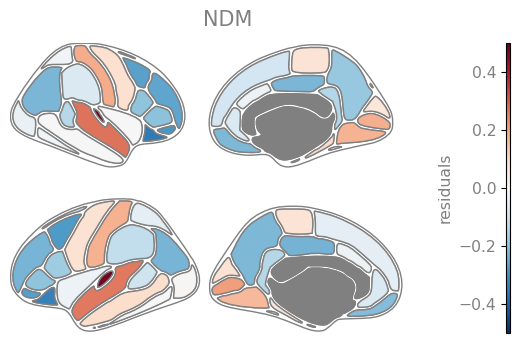
\includegraphics[width=\linewidth]{residuals_ndm_cn.png}
%         \vspace{1mm}
%         \textbf{(a)}
%     \end{subfigure}
%     \hfill
%     \begin{subfigure}[b]{0.45\linewidth}
%         \centering
%         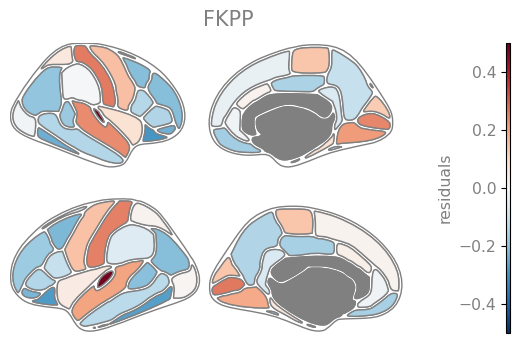
\includegraphics[width=\linewidth]{residuals_fkpp_cn.png}
%         \vspace{1mm}
%         \textbf{(b)}
%     \end{subfigure}
%     \vskip 4mm
%     \begin{subfigure}[b]{0.45\linewidth}
%         \centering
%         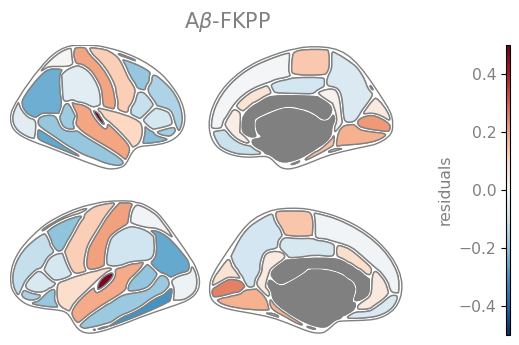
\includegraphics[width=\linewidth]{residuals_wfkpp_cn.png}
%         \vspace{1mm}
%         \textbf{(c)}
%     \end{subfigure}
%     \hfill
%     \begin{subfigure}[b]{0.45\linewidth}
%         \centering
%         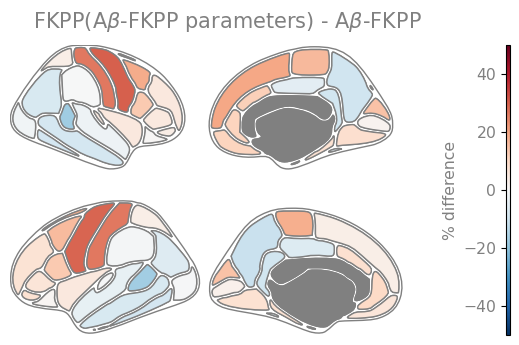
\includegraphics[width=\linewidth]{residuals_fkpp_wfkpp_diff_cn.png}
%         \vspace{1mm}
%         \textbf{(d)}
%     \end{subfigure}
%     \caption{Residuals from NDM, FKPP, A$\beta$-FKPP (panels a--c) and the difference between weighted-FKPP and FKPP (panel d).}
%     \label{fig:comparison_subfigures}
% \end{figure}

\subsubsection{Robustness testing through individual connectome analysis}
Though the NDM fit to group average connectome had better r values, we observed that the mean performance across individuals had the largest (negative) difference compared to other models, and had the largest 95 percentile ranges. The NDM also had the largest 95 percentile range of SSE values across individuals, indicating that the model fit was not robust across individuals.\\ 

A$\beta$-FKPP model had generally worse performance mean across individuals, but this may be attributable to using group-averaged A$\beta$-FKPP values that aligned better with group-averaged connectomes, and it would be interesting to see if the model fit improves when using individual A$\beta$-FKPP values.


\begin{table*}[h]
    \centering
    \small % Reduce font size slightly
    \setlength{\tabcolsep}{4pt} % Reduce column spacing
    \caption{Model performance distribution across individual connectomes}
    \label{tab:model_performance_distribution_individuals}
    \begin{tabular}{lccccccccc}
    \toprule
    & & \multicolumn{4}{c}{\textbf{SSE}} & \multicolumn{4}{c}{\textbf{Pearson's r}} \\
    \cmidrule(lr){3-6} \cmidrule(lr){7-10}
    \textbf{Group} & \textbf{Model} & \textbf{Avg} & \makecell{\textbf{Indiv.} \\ \textbf{$\mu$}} & \makecell{\textbf{\%} \\ \textbf{diff}} & \makecell{\textbf{95p Range}} & \textbf{Avg} & \makecell{\textbf{Indiv.} \\ \textbf{$\mu$}} & \makecell{\textbf{\%} \\ \textbf{diff}} & \makecell{\textbf{95p Range}} \\
    \midrule
    \rowcolor{gray!15}
    CN & NDM & 2.48 & 2.50 & 0.64 & 0.555 & 0.724 & 0.677 & \textbf{-6.97} & 0.168 \\
    \rowcolor{gray!15}
    CN & FKPP & 2.25 & 2.26 & 0.45 & 0.352 & 0.667 & 0.655 & -1.69 & 0.091 \\
    \rowcolor{gray!15}
    CN & A$\beta$-FKPP & 1.86 & 1.90 & \textbf{2.14} & 0.394 & 0.720 & 0.718 & -0.36 & 0.151 \\
    \midrule
    EMCI & NDM & 2.53 & 2.56 & 1.04 & \textbf{0.630} & 0.719 & 0.686 & -4.80 & \textbf{0.174} \\
    EMCI & FKPP & 2.30 & 2.29 & -0.36 & 0.348 & 0.663 & 0.654 & -1.36 & 0.091 \\
    EMCI & A$\beta$-FKPP & 1.88 & 1.92 & 1.90 & 0.453 & 0.713 & 0.715 & 0.20 & 0.113 \\
    \midrule
    \rowcolor{gray!15}
    LMCI & NDM & 2.62 & 2.60 & -0.53 & 0.604 & 0.718 & 0.654 & \textbf{-9.76} & \textbf{0.174} \\
    \rowcolor{gray!15}
    LMCI & FKPP & 2.33 & 2.35 & 0.83 & 0.468 & 0.654 & 0.641 & -2.03 & 0.110 \\
    \rowcolor{gray!15}
    LMCI & A$\beta$-FKPP & 1.93 & 1.96 & 1.44 & \textbf{0.662} & 0.709 & 0.706 & -0.43 & 0.141 \\
    \midrule
    AD & NDM & 2.56 & 2.61 & \textbf{1.87} & \textbf{0.809} & 0.714 & 0.656 & \textbf{-8.97} & \textbf{0.231} \\
    AD & FKPP & 2.32 & 2.32 & 0.16 & 0.505 & 0.662 & 0.645 & -2.69 & 0.126 \\
    AD & A$\beta$-FKPP & 1.91 & 1.95 & \textbf{2.09} & 0.426 & 0.712 & 0.708 & -0.58 & 0.116 \\
    \bottomrule
    \end{tabular}
\end{table*}

\subsection{Using optimal hyperparameters from the A$\beta$-FKPP model on FKPP}
The FKPP model, when forced to use the A$\beta$-FKPP model’s optimal parameters, sees an increase in SSE from 1.86 to 2.40, and a decrease in r score from 0.72 to 0.62.
We see an increase in predicted tau deposition in the Precentral and Postcentral regions, but a decrease in Bankssts and the Inferiortemporal regions. This divergence from pure FKPP suggests that the A$\beta$-modulated seed choice and growth rate emphasize certain pathways in a way that does not neatly translate into the unweighted FKPP environment. These findings underscore that parameters valid in a model incorporating amyloid load may not fully transfer to a simpler model, highlighting the importance of explicitly accounting for amyloid–tau interactions to better capture disease progression patterns.

\begin{figure}[h]
    \centering
    % First subfigure: The image
    \begin{subfigure}[b]{\linewidth}
        \centering
        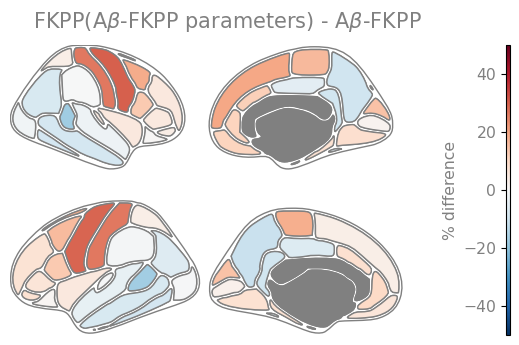
\includegraphics[width=\linewidth]{residuals_fkpp_wfkpp_diff_cn.png}
        \caption{Prediction difference between FKPP with A$\beta$ parameters versus A$\beta$-FKPP.}
        \label{fig:fkpp_wfkpp_diff}
    \end{subfigure}
    
    \vspace{1em} % Optional vertical space to separate the subfigures
    
    % Second subfigure: The table with mandatory width argument added
    \begin{subfigure}[b]{\linewidth}
        \centering
        \begin{tabular}{c|p{2.7cm}|p{1.5cm}}
            \toprule
                & \textbf{Regions} & \textbf{\% Diff} \\
            \midrule
            \multirow{3}{*}{%
                \parbox{2.3cm}{\centering \textbf{FKPP}\\ \textbf{higher}}
            }
                & \textcolor{red}{Precentral L} & 29.7\\
                & \textcolor{red}{Postcentral L} & 29.2\\
                & \textcolor{red}{Precentral R} & 26.4\\ 
            \midrule
            \multirow{3}{*}{%
                \parbox{2.3cm}{\centering \textbf{A$\beta$-FKPP}\\ \textbf{higher}}
            }
                & \textcolor{blue}{Bankssts L} &17.6\\
                & \textcolor{blue}{Bankssts R} &17.2\\
                & \textcolor{blue}{Inferiortemporal R} &11.2\\
            \bottomrule
        \end{tabular}
        \caption{Top 3 regions with largest differences between models}
        \label{tab:fkpp_wfkpp_diff}
    \end{subfigure}
    
\end{figure}

    
    

\subsection{Influence of A$\beta$ on tau production}
The null model performs significantly worse (permutation-based p-value $<$ 0.01), thus concluding that ground truth A$\beta$ is the key factor for A$\beta$-FKPP's performance. What's most interesting is the inclination towards Inferiortemporal regions as the optimal seed, which corresponds also to the optimal seeds in NDM and FKPP models, meanwhile the original Entorhinal seed was never selected.
\begin{figure}[h]
    \centering
    \begin{subfigure}[t]{0.4\linewidth}
        \centering
        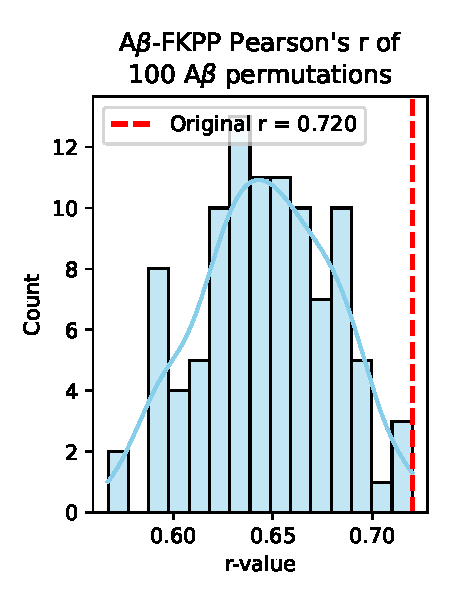
\includegraphics[width=\linewidth]{wfkpp_permuted_ab_r_distribution.pdf}
        \vspace{1mm}
        \textbf{(a)}
    \end{subfigure}
    \begin{subfigure}[t]{0.55\linewidth}
        \centering
        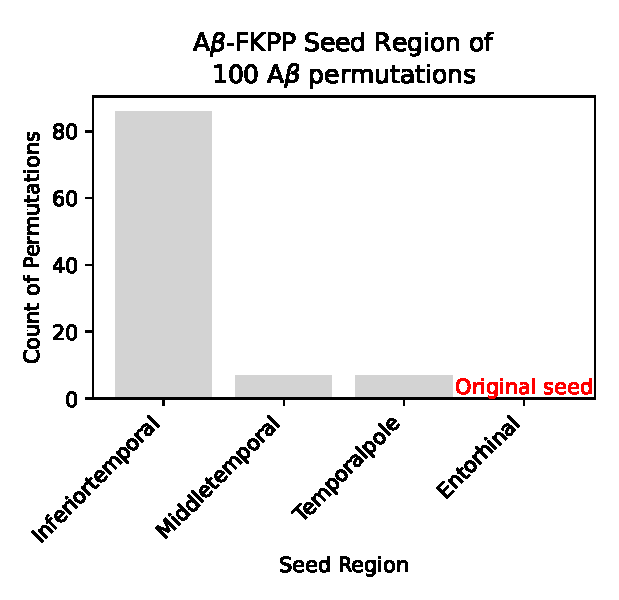
\includegraphics[width=\linewidth]{wfkpp_permuted_ab_seed_region.pdf}
        \vspace{1mm}
        \textbf{(b)}
    \end{subfigure}
    \caption{Distribution of r values when permuting the A$\beta$ weights (a) and The distribution of optimal seed regions across 100 permutations (b).}
    \label{fig:null_model_permute_ab}
\end{figure}

\subsection{The effect of the best performing cognitive group on FKPP and NDM}
In both FKPP and NDM, the null models perform significantly worse, with the best connectome a large margin away from the original, thus verifying that the original connectome is a key factor for the best performing group average connectome's performance. We also see a more diverse set of optimal seed regions chosen.
\begin{figure}[h]
    \centering
    \begin{subfigure}[t]{0.4\linewidth}
        \centering
        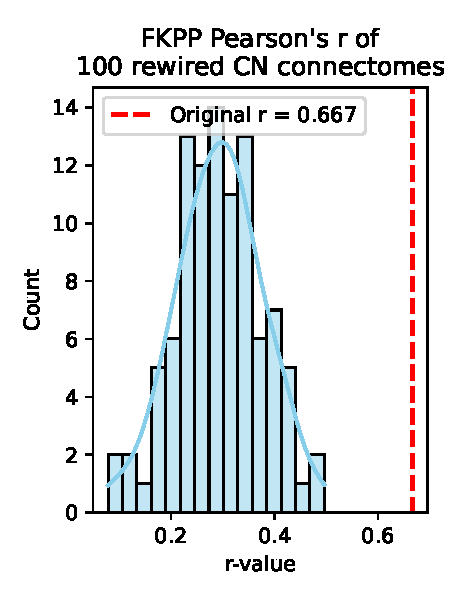
\includegraphics[width=\linewidth]{fkpp_rewired_r_distribution.pdf}
        \vspace{1mm}
        \textbf{(a)}
    \end{subfigure}
    \begin{subfigure}[t]{0.55\linewidth}
        \centering
        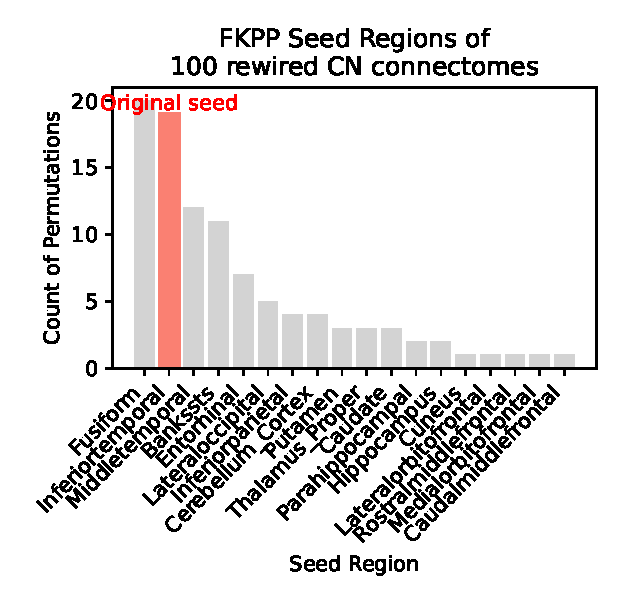
\includegraphics[width=\linewidth]{fkpp_rewired_seed_region.pdf}
        \vspace{1mm}
        \textbf{(b)}
    \end{subfigure}
    \vskip 4mm
    \begin{subfigure}[t]{0.4\linewidth}
        \centering
        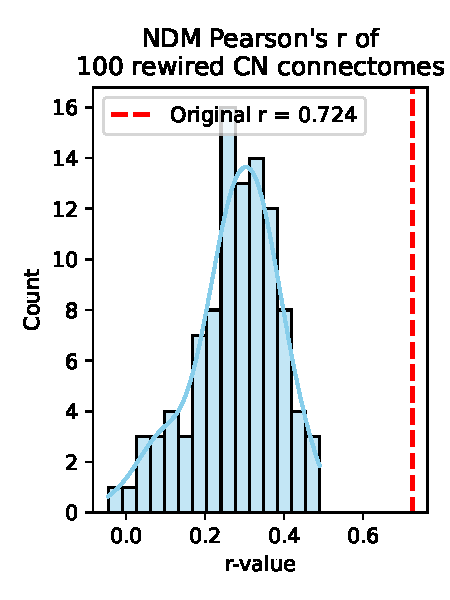
\includegraphics[width=\linewidth]{ndm_rewired_r_distribution.pdf}
        \vspace{1mm}
        \textbf{(c)}
    \end{subfigure}
    \begin{subfigure}[t]{0.55\linewidth}
        \centering
        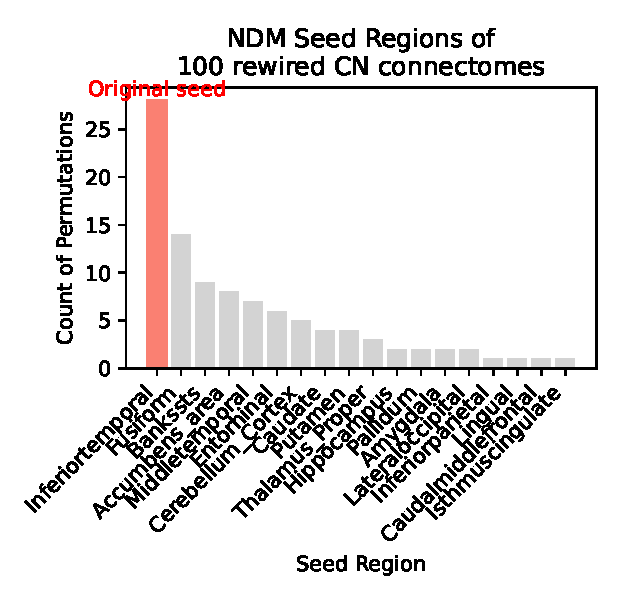
\includegraphics[width=\linewidth]{ndm_rewired_seed_region.pdf}
        \vspace{1mm}
        \textbf{(d)}
    \end{subfigure}
    \caption{Distribution of r values when rewiring connectomes (a) and The distribution of optimal seed regions across 100 permutations (b).}
    \label{fig:null_model_rewire_connectomes}
\end{figure}



